\section{\methodfull}
\label{sec:method}

\methodfull (\method) treats every position at every denoising step as a per-position decision: \emph{keep} the current token, \emph{re-mask} it to \mask\ for re-prediction, or, if currently masked, \emph{reveal} a new token. We present \method\ in the following parts: the inference decision rule that maps model probabilities to per-position keep / re-mask / reveal actions (\S\ref{sec:inference}); 
\temporalmethodfull (\temporalmethod), a parameter-free per-position history aggregation mechanism that summarizes the denoising trajectory into a history-aware embedding for the model (\S\ref{sec:temporal-residual});
the training objective that enables models' \methodfull capability and the recipe used to construct training inputs (\S\ref{sec:training}).



\textbf{Notations.} Let $\xstar \in \mathcal{V}^N$ denote the target sequence and $E \subseteq \{1, \ldots, N\}$ the set of editable positions  (full sequence excluding the instruction prompt). For each $i \in E$, the position can take one of three values throughout the denoising trajectory:
$\tilde{x}^{(t)}_i \;\in\; \{w_i, \mask, \xstar_i\}$
where $w_i$ is a task-specific wrong token. Non-edit positions $i \notin E$ stay at $\xstar_i$ at every step. We write $T$ for the total number of denoising steps and $\bar{\mathcal{V}} := \mathcal{V} \cup \{\mask\}$ for the extended vocabulary.



\subsection{Basic inference rules on MDMs with \methodfull enabled}
\label{sec:inference}



Unlike the standard MDM inference rule, which follows an absorbing Markov process, we introduce \methodfull that allows the model to revisit and revise past decisions, enabling test-time scaling. To enable this, we define a new inference rule. At timestep $t \in \{0, 1, \ldots, T-1\}$ the model takes the current state $\tilde{x}^{(t)}$ as input and outputs a per-position categorical $p_\theta(\cdot \mid \tilde{x}^{(t)})_i$ over $\bar{\mathcal{V}}$. The next-step state is then determined per position by a deterministic rule that splits on whether the position is currently non-mask or masked. $\mask$ is denoted as M:
\begin{equation}
\tilde{x}^{(t+1)}_i =
\begin{cases}
M
& \text{if } \tilde{x}^{(t)}_i \neq M \text{ and } p_\theta(M \mid \tilde{x}^{(t)})_i > p_\theta(\tilde{x}^{(t)}_i \mid \tilde{x}^{(t)})_i \; \textit{\text{(\method),}} \\[4pt]
\tilde{x}^{(t)}_i
& \text{if } \tilde{x}^{(t)}_i \neq M \text{ and } p_\theta(M \mid \tilde{x}^{(t)})_i \leq p_\theta(\tilde{x}^{(t)}_i \mid \tilde{x}^{(t)})_i \; \textit{\text{(Keep),}} \\[4pt]
\displaystyle \arg\max_{v \in \mathcal{V}}\, p_\theta(v \mid \tilde{x}^{(t)})_i
& \text{if } \tilde{x}^{(t)}_i = M \; \textit{\text{(Reveal).}}
\end{cases}
\label{eq:remask-rule}
\end{equation}

The rule is intuitive. At a non-mask position, re-mask whenever the model assigns higher probability to \mask\ than to the current token, because the model is signaling that the non-mask token is wrong; otherwise keep it. At a \mask\ position, reveal the most likely vocabulary token. In general, at each iteration, model can produce one of three actions per position: keep, re-mask, or reveal, all driven entirely by the model’s per-position output distribution.


This basic rule as presented conditions only on the current state $\tilde{x}^{(t)}$. As a result, the model may produce the same state across different time steps, leading to a loop where identical states are repeatedly passed to subsequent steps. We address this in \S\ref{sec:temporal-residual} by changing what the model sees as input, while leaving Eq.~\eqref{eq:remask-rule} unchanged.
\subsection{Enhancing \methodfull with \temporalmethodfull }
\label{sec:temporal-residual}

\begin{wrapfigure}[16]{r}{0.6\linewidth}
\centering
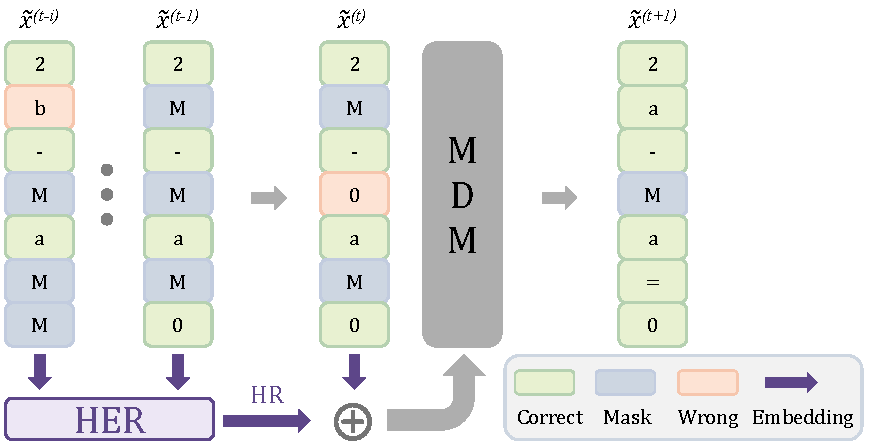
\includegraphics[width=0.9\linewidth]{figures/inference_main_paper.pdf}
\caption{\textbf{Inference procedure with \temporalmethodfull.} All states are embedded, and the historical states are further processed by HER. The embedding of current step $\tilde{x}^{(t)}$ is added to the history reference (HR) and fed into the model as the input, which predicts the next step $\tilde{x}^{(t+1)}$.}
\label{fig:inference-dataflow}
\end{wrapfigure}

To let the model condition on more than the current state, we maintain a per-position accumulated embedding that compresses the prefix $\tilde{x}_i^{(0:t)}$ into a single vector and feed it to the model. The accumulated embedding adds no learnable parameters and admits an $O(1)$ per-step update (Appendix~\ref{app:rope-engineering}).

\paragraph{Setup.}
Let $e_i^{(k)} := \mathrm{wte}(\tilde{x}_i^{(k)})$ denote the model token embedding of position $i$ at step $k$. Let $R_\Delta$ denote the \emph{\distancemethodfull (\distancemethod)} indexed by the distance $\Delta = k - t$ between a historical step $k$ and the current step $t$, satisfying the standard rotation composition rules
\[
R_0 = I, \qquad R_a R_b = R_{a+b}, \qquad R_{-\Delta} = R_\Delta^{\top}.
\]
$R_\Delta$ is a parameter-free block-diagonal rotation that applies a distance to each two-dimensional block of an embedding. We instantiate it with the same two-dimensional sinusoidal blocks used by standard rotary encodings~\citep{su2024roformer}.

\paragraph{History embedding.}
At iteration $t$ we express every historical state in the current step's reference frame and accumulate them into a single vector:
\begin{equation}
a_i^{(t)} \;=\; \sum_{k=0}^{t} \gamma^{\,t-k}\, R_{k-t}\, e_i^{(k)},
\label{eq:temporal-embedding}
\end{equation}
where $\gamma \in (0, 1]$ is a history-decay factor. Equivalently,
\[
a_i^{(t)} \;=\; e_i^{(t)} + \gamma\, R_{-1}\, e_i^{(t-1)} + \gamma^{2}\, R_{-2}\, e_i^{(t-2)} + \cdots + \gamma^{t}\, R_{-t}\, e_i^{(0)}.
\]
The current state contributes unrotated, while each past state is added with a lag-dependent rotation \(R_\Delta\) and decay \(\gamma^{|\Delta|}\). Two sequences that share the same current state are augmented by their histories, which provide additional conditioning signals. This historical context allows the model to reference past states when deciding whether to re-mask or keep a token, helping it avoid recurring errors and leverage useful cues from earlier versions.



\subsection{Training paradigm for enabling \methodfull in MDMs}
\label{sec:training}

To enable the model to follow the inference rule of \S\ref{sec:inference}--\S\ref{sec:temporal-residual}, we design a training paradigm that aligns its per-position outputs with the correct next-step actions. Concretely, we train the model with per-position oracle labels, encouraging its output distribution to assign the highest probability to the desired next action at each position.

\paragraph{Oracle revision rule.}
For each $i \in E$ and any state $z_i \in \{w_i, \mask, \xstar_i\}$, the optimal next-step action is the deterministic function
\begin{equation}
\tau(z_i, \xstar_i) \;=\; \begin{cases}
\mask & z_i \in \mathcal{V} \setminus \{\xstar_i\} \quad \text{(re-mask wrong / initial token)} \\
\xstar_i & z_i = \mask \quad \text{(reveal target)} \\
\xstar_i & z_i = \xstar_i \quad \text{(preserve target).}
\end{cases}
\label{eq:oracle-tau-method}
\end{equation}
A non-mask token that differs from the target should be re-masked, a \mask\ should be revealed to the target, and a correct non-mask token should be preserved. Non-edit positions are deterministically labelled $\xstar_i$ at every step.

\paragraph{Training data curation.}
\begin{figure}[t]
    \centering
    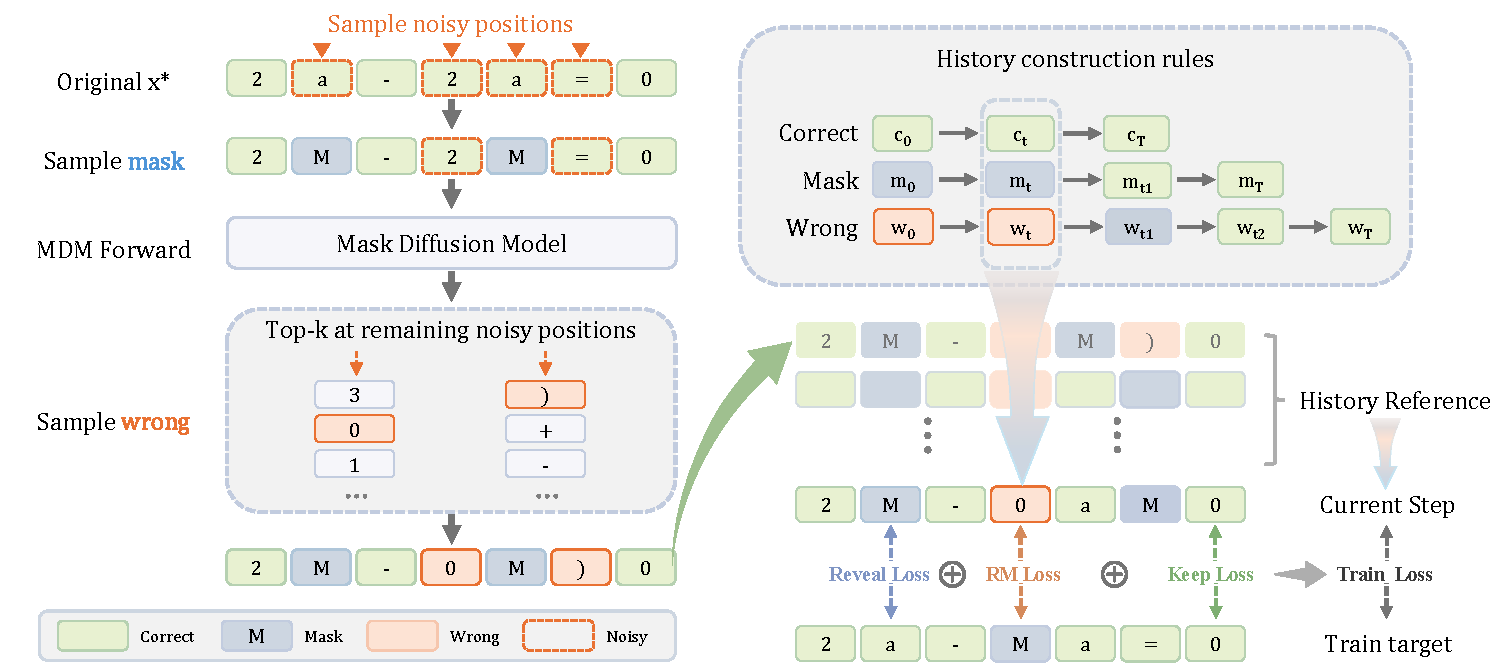
\includegraphics[width=\linewidth]{figures/data_synthetic_train_main_paper_v3.pdf}
    \caption{\textbf{Synthetic history data construction for Mask Diffusion Model Training}.
    A noisy sequence is created from a clean sequence using mask and wrong-token corruption. Position-wise transition rules are then used to sample synthetic histories and define training targets.}
    \label{fig:data_synthetic_pipe}
\end{figure}
As illustrated in Fig.~\ref{fig:data_synthetic_pipe}, a training instance is constructed by simulating a synthetic trajectory, starting from an original clean sequence $\xstar$. We first sample a subset of positions to corrupt and draw a timestep $t \sim \mathrm{Uniform}\{0, \ldots, T-1\}$. At this timestep, the selected positions are split into two groups: one is replaced with \mask\ tokens, while the other is substituted with wrong tokens. Wrong tokens are sampled from a corruption distribution $\nu(\cdot \mid \xstar_i)$ over $\mathcal{V} \setminus \{\xstar_i\}$. In practice, $\nu$ is chosen to better match inference-time errors, e.g., using top-$k$ predictions from a frozen MDM backbone (excluding the ground-truth token) or task-specific token distributions. Appendix~\ref{app:topk-tv-gap} bounds the resulting shift of the training objective relative to a uniform proposal. This yields the current state $z = \tilde{x}^{(t)}$.

To approximate inference-time dynamics, we construct histories following position-wise transition rules (right side of Fig.~\ref{fig:data_synthetic_pipe}). Each position evolves independently according to its current state: correct tokens remain unchanged; masked tokens transition to correct tokens at a sampled timestep $t_1$; and wrong tokens first transition to mask tokens at sampled timestep $t_1$ and then to correct tokens at later timestep $t_2$. These transitions are governed by per-position rules together with sampled transition timesteps within the $T$-step horizon, which jointly define the trajectory sampler.

Sampling these transition timesteps produces a set of reference states that mimic iterative refinement during inference. Based on the resulting state, training targets are defined per position: masked tokens are trained to predict the correct token, while wrong tokens are trained to predict the mask token. The overall objective combines reveal, mask, and keep losses. This construction defines a trajectory sampler that specifies the training input distribution, while remaining independent of model parameters $\theta$, providing a stable target for optimization. The full procedure is given in Appendix~\ref{app:training-algo}.

\paragraph{Training objective.}
The model receives $a^{(t)}$ and outputs per-position categorical distributions. We supervise each position using an oracle action $\tau(z_i, \xstar_i)$ that depends on its current state: masked tokens are mapped to their correct token (reveal), wrong tokens are mapped to \mask\ (mask), and correct tokens are kept unchanged (keep).

We minimize the per-position cross-entropy against this oracle,
\begin{equation}
\Ltrain(\theta) \;=\; \mathbb{E}\!\left[\,\sum_{i \in E} -\log p_\theta\!\left(\tau(z_i, \xstar_i) \,\big|\, a^{(t)}\right)_i\right],
\label{eq:total-loss}
\end{equation}
where the expectation is over the data distribution, the random trajectory and step sampling.

Equivalently, the objective decomposes into three components:
a \textit{reveal loss}, which predicts the correct token for masked positions;
a \textit{mask loss}, which predicts \mask\ for wrong positions;
and a \textit{keep loss}, which preserves correct tokens.
This decomposition matches the training targets induced by the synthetic trajectory construction in Fig.~\ref{fig:data_synthetic_pipe}.

Two properties of this objective justify its use. First, given a sufficiently expressive model, minimizing Eq.~\eqref{eq:total-loss} drives the model's per-input output toward the conditional distribution of the oracle action $\tau$, so the argmax of the trained model recovers the inference rule of Eq.~\eqref{eq:remask-rule}. Second, conditioning on $a^{(t)}$ instead of the bare current state $\tilde{x}^{(t)}$ cannot increase the optimal training risk, since a richer input representation can only improve (or leave unchanged) the best achievable expected loss. Please refer to Appendix~\ref{app:theory} for the complete theoretical justification and detailed proofs.